%  \enlargethispage{2cm}
\section{Enzymes are essential to life}\label{sec:Enzymes}
	\begin{quote}
	Enzymes speed up reactions which otherwise wouldn't take place in a cell \\
	Enzymes allow for life at relatively low temperatures \\ 
	Enzymes may be called "`working proteins"'\\
	Enzymes are susceptible to conditions of pH or salinity within a cell \\
	Enzymes can be positively regulated - "`activated"' \\
	Enzymes can be negatively regulated - "`inhibited"'
	\end{quote}
	
\subsubsection*{Enzymes' BrainStorm}
\Kommentar{ 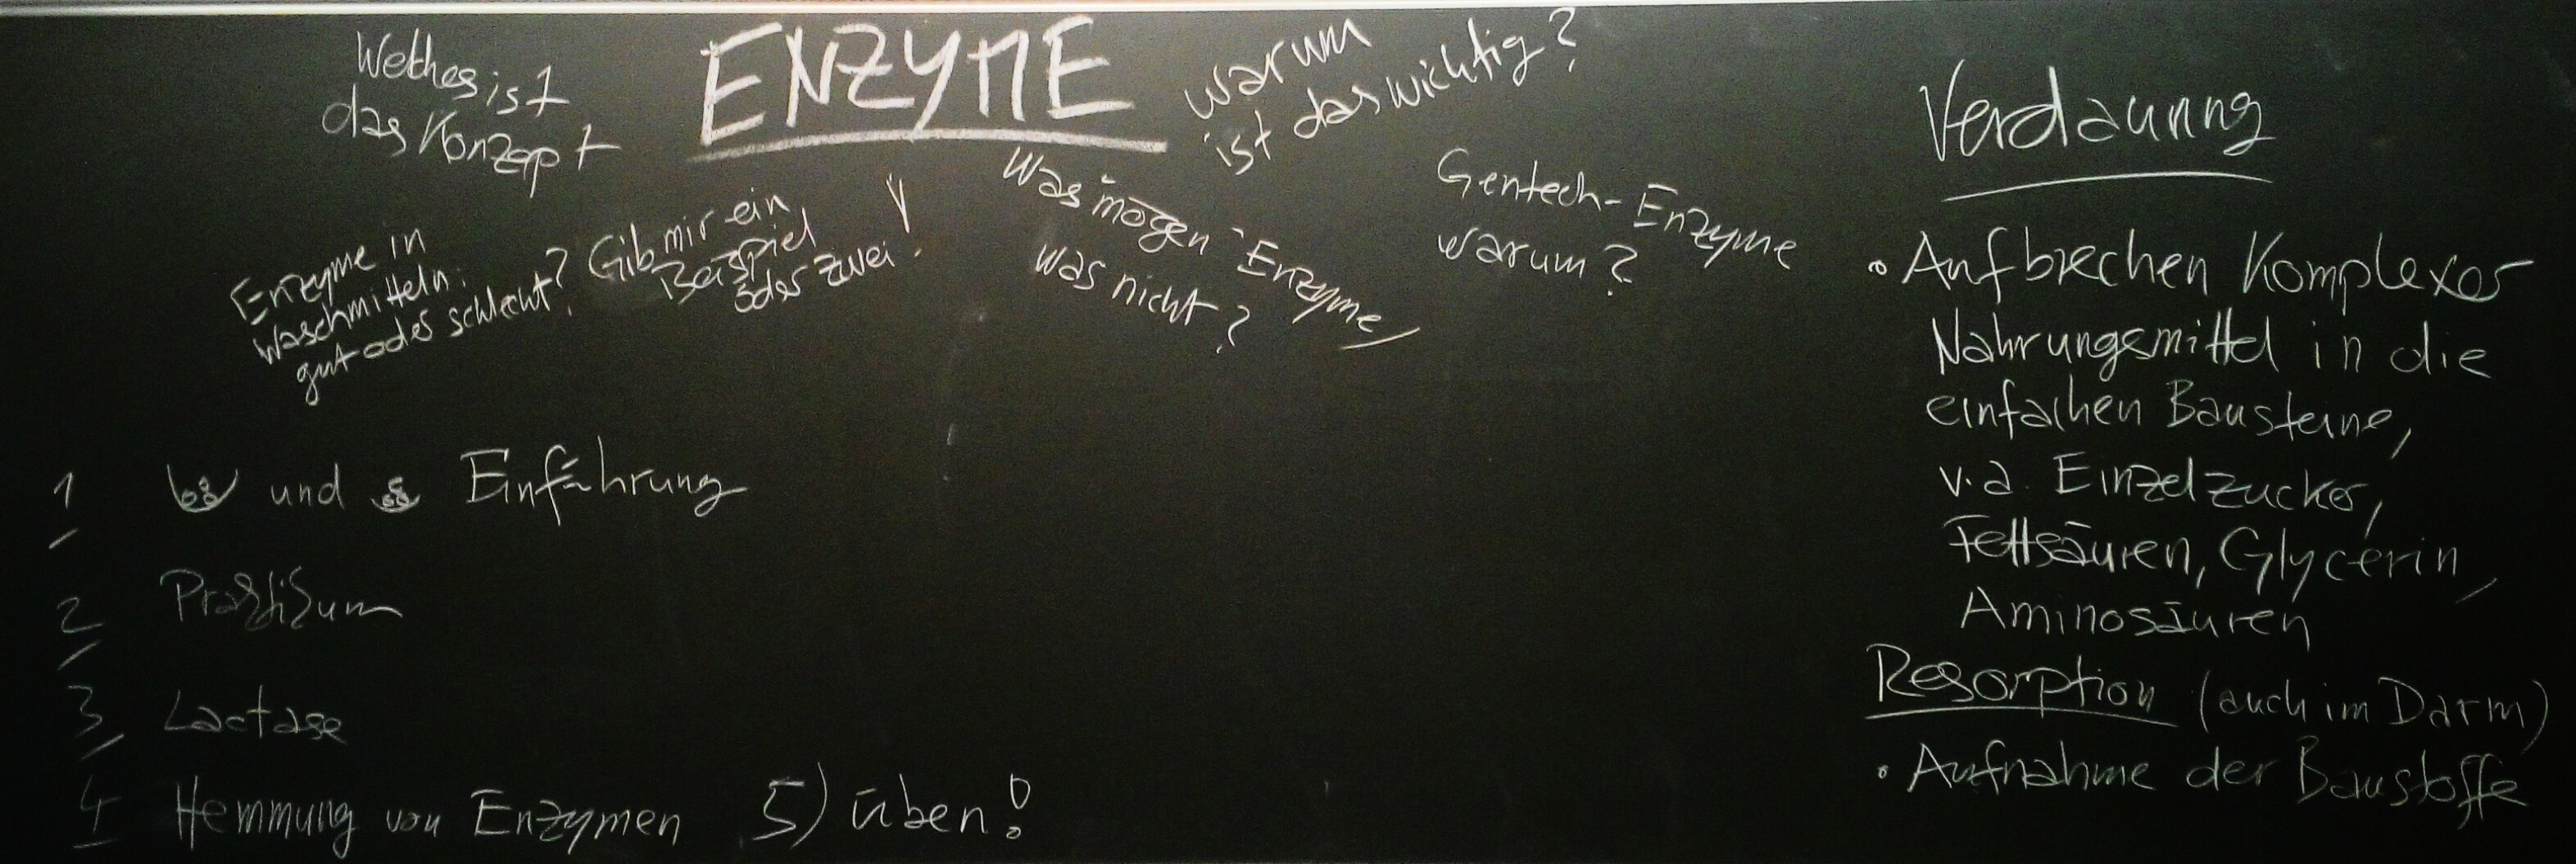
\includegraphics[width=12cm]{/share/Dropbox/Kamera-Uploads/20181029_155010626.jpg}
		}{}{6cm}{}

\subsubsection*{Enzymes in a nutshell}
\Kommentar{ 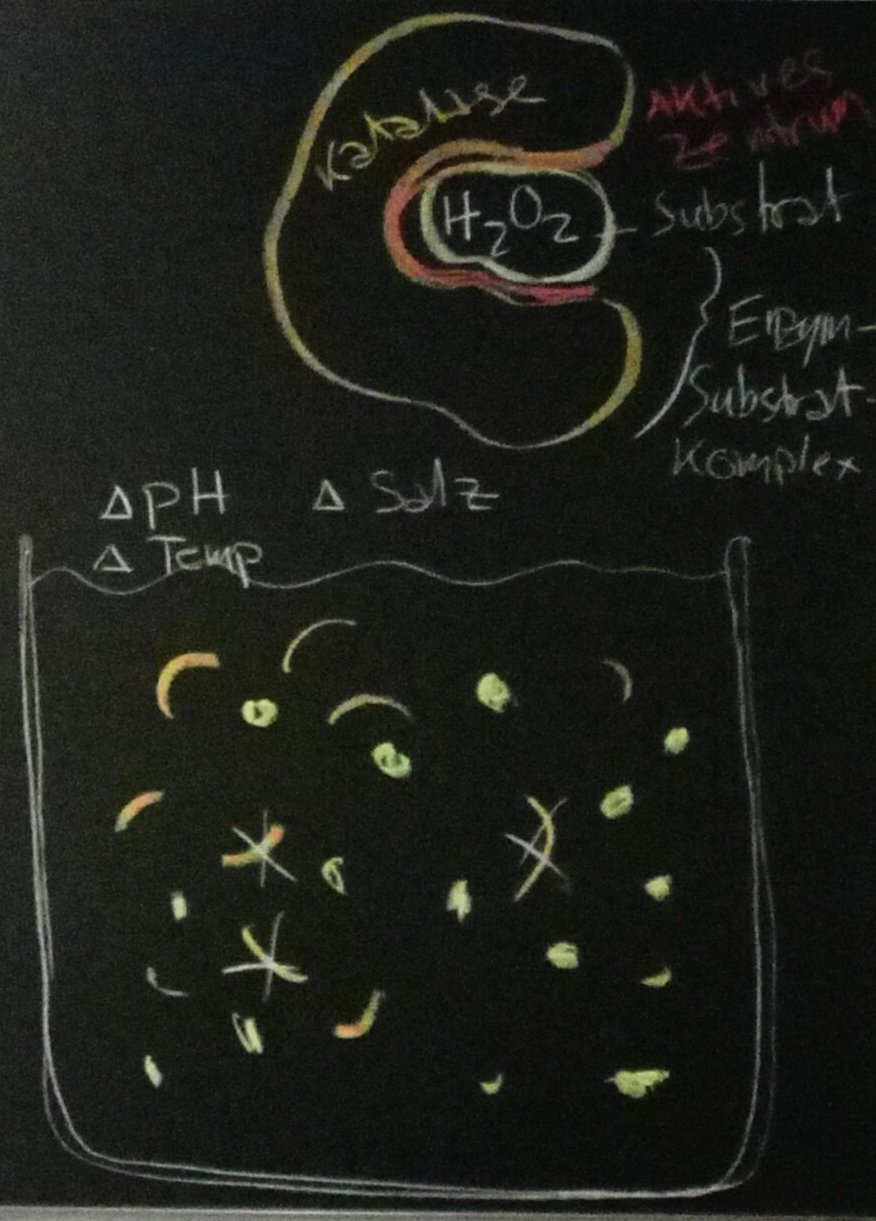
\includegraphics[width=4cm]{/share/SB_Unterricht/Biologie/met02_Enzyme/20181102_092820430_v1.png}
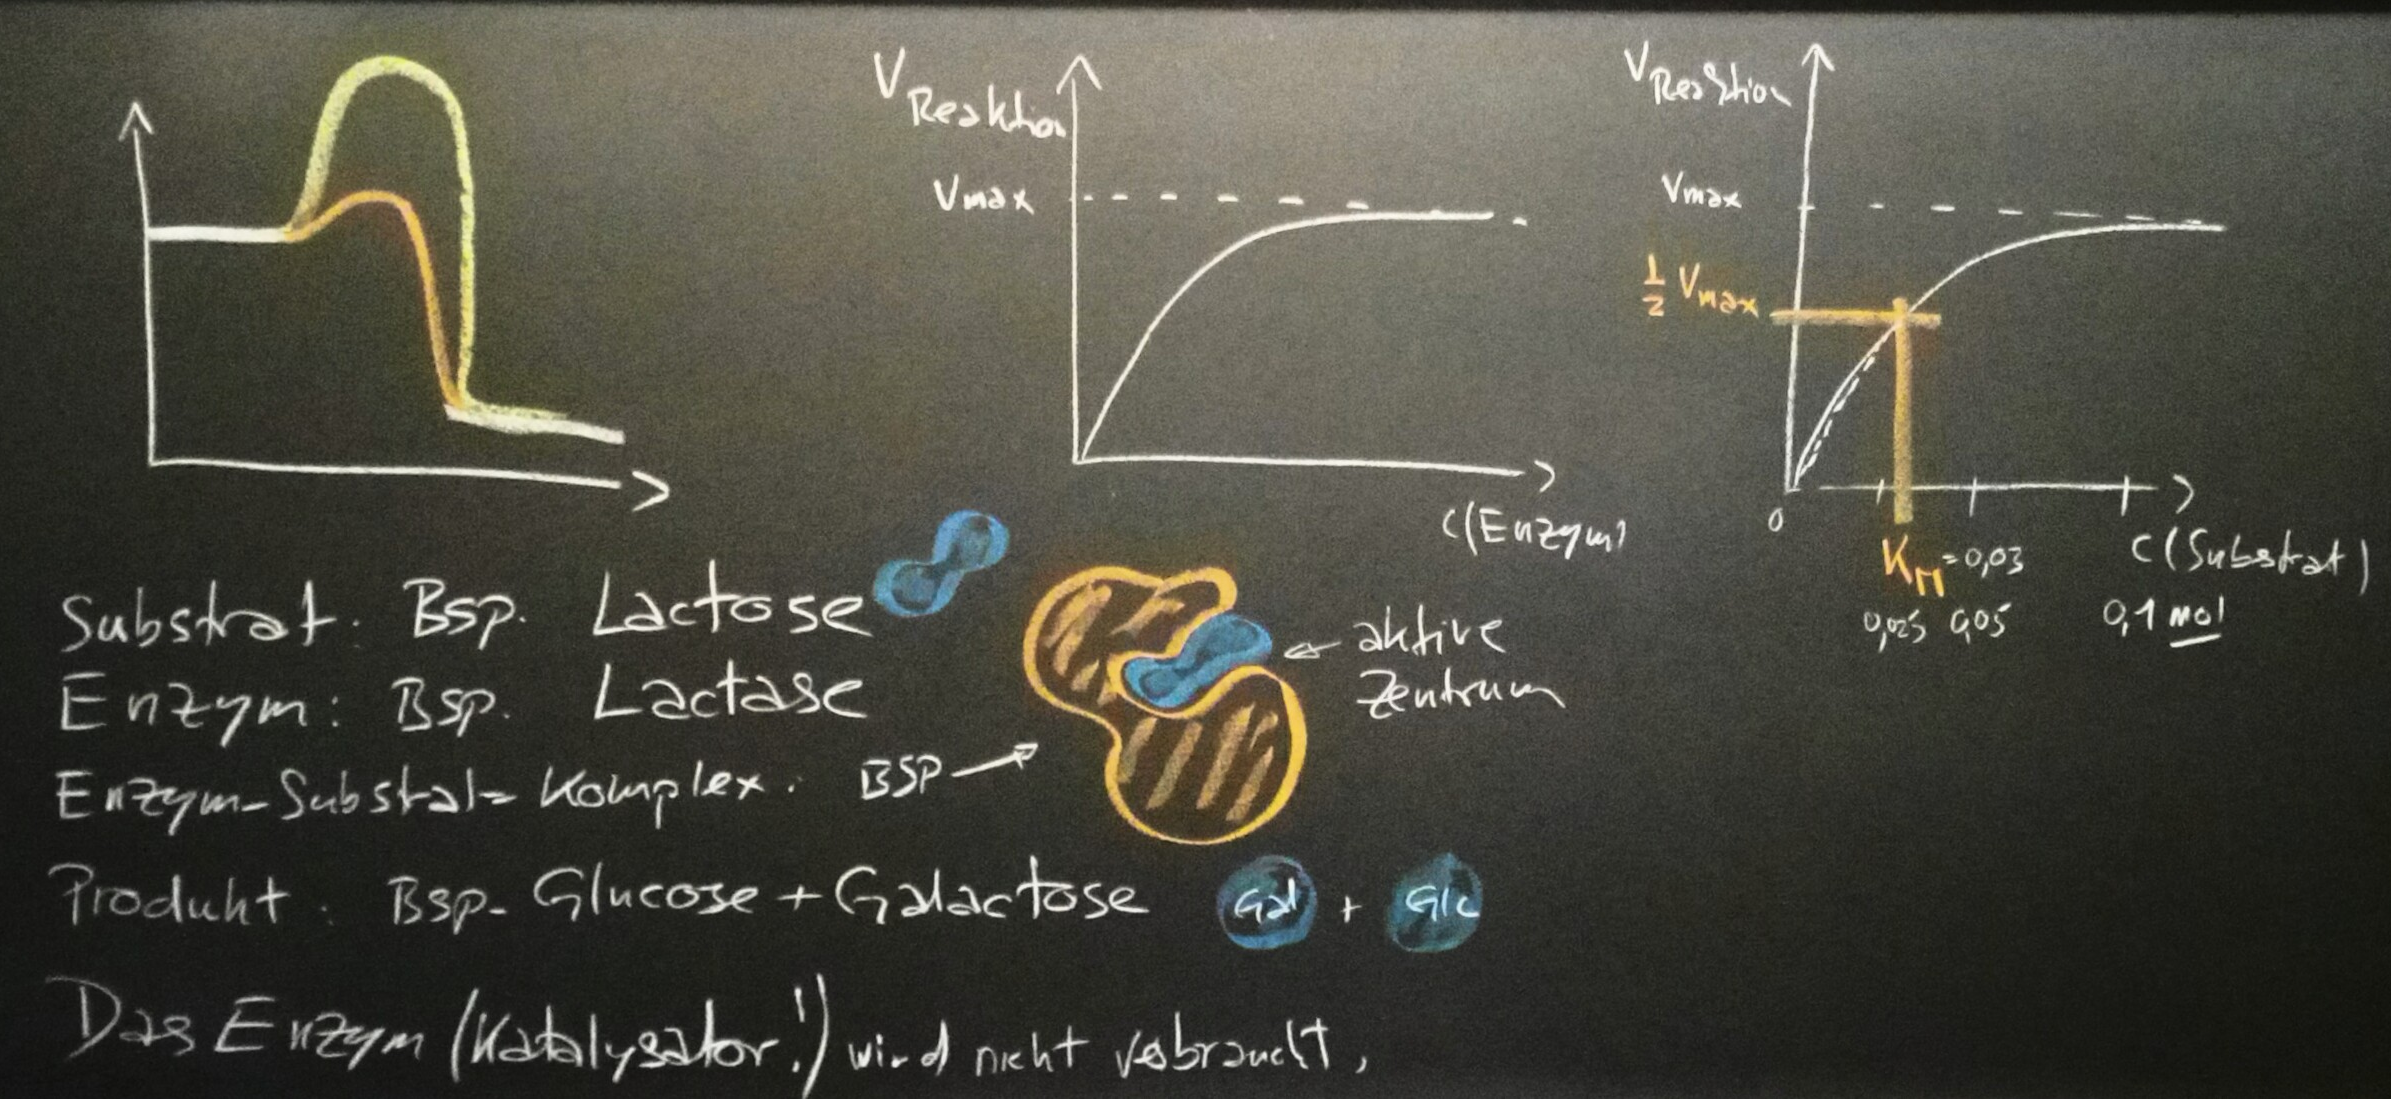
\includegraphics[width=8cm]{/share/SB_Unterricht/Biologie/met02_Enzyme/20181030_113931359_v1.png}
		}{}{8cm}{}

\clearpage
\subsection{Introductory experiment with lactase tablets}
	\begin{marginfigure}[1cm]%
		\hspace{1cm}  \includegraphics[width=2.5cm]{/share/SB_Unterricht/Biologie/met02_Enzyme/Lactase-Intoleranz/Milch-Emmi-Tetrapack.jpeg}
	 \end{marginfigure}

Do you like drinking milk, without any amendments such as chocolate? If you say "`no"' your body might give you a warning: a quarter of the Europeans are unable to digest \textbf{lactose}, milk sugar. The problem here is \emph{conveniance food} and the addition of milk sugar in countless food products, from "`Aromat"', to pralinés, power bars, Fasnachtschüechli or even ordinary bread. The inability to digest lactose can lead to diarrhoea, stomach cramps and more. The cause is genetically encoded: lactose intolerant people lack a mutation enabling many Europeans (but only about 5\% of Asians) to produce the enzyme \textbf{lactase} longer than the breast feeding period (toddlers up to three years).



\begin{enumerate}[itemsep=1.5em, leftmargin=*]
\item  Glucose test strips may be used to observe the activity of the \textbf{enzyme lactase}. Use the world cloud to \emph{describe} the experiments shown in class!
\end{enumerate}
\begin{marginfigure}[0pt]%
  \includegraphics[width=\linewidth]{/share/SB_Unterricht/Biologie/met02_Enzyme/Lactase-Intoleranz/Lactase-Wirkung_vonNovartisSkript.png}
%   \caption[VERZEICHNIS]{CAPTION}
%   \label{fig:LABEL}
\end{marginfigure}

\hspace{1.4cm}
\includegraphics[width=7cm]{/share/SB_Unterricht/Biology/met02_enzymes/lactase-wordcloud.png}

%%%%%%%%%%%%%%%%%%%%%%%%%%%%%%%%%%%%%%%%
% % I used these words in \url{https://worditout.com/word-cloud/create}
% % 	lactose lactose lactose lactose  lactose lactose
% % 	lactase lactase lactase lactase lactase lactase lactase lactase lactase
% % 		0.5%-lactose-solution 0.5%-lactose-solution 0.5%-lactose-solution
% % 		tap-water  tap-water  tap-water
% % 		grind grind
% % 		mortar-with-pistil mortar-with-pistil
% % 		incubation incubation
% % 		37°C  37°C
% % 	enzyme enzyme enzyme enzyme
% % 	glucose glucose glucose
% % 	galactose galactose galactose
% % 	separation separation separation
% % 	enzyme-substrate-complex
% % 	cleavage
% % 	disccharide  monosaccharide
% % 	glucose-test-strips glucose-test-strips glucose-test-strips glucose-test-strips glucose-test-strips
% % 	mmol-per-litre mmol-per-litre
% % 	increase increase
% % 	value value
% % 	measurement
% % 	-ase -ase -ase
% % 	milk milk milk milk milk milk milk
% % 	lactose-free-milk lactose-free-milk  lactose-free-milk lactose-free-milk lactose-free-milk
%%%%%%%%%%%%%%%%%%%%%%%%%%%%%%%%%%%%%%%%


 \areaset[0cm]{15cm}{28cm}
\subsection{The Starr read on the priniciples of energy conversion}
%  \thispagestyle{empty}
		\begin{mdframed}[style=exampledefault, userdefinedwidth=12cm,frametitle={Starr chapters 5.1, 5.2, 5.3, 5.4}\label{mat:BEISPIELMATERIAL}]	  
			Starr placed the enzymes at the beginning of his book: they are essential to life, allowing for the conversion of either energy or any biochemichal molecules. (see \textit{Mrs Gren, the criteria of life}!)
		\end{mdframed}
	
\begin{enumerate}[itemsep=1.2em, leftmargin=*]
	\item  From \ding{229} Starr chapter 5.1, summarise the \emph{first law of thermodynamics}: \\
		\Loesung{... read it from the book... \fillwithdottedlines{1cm}}{1.7cm}
		
	\item  From \ding{229} Starr chapter 5.1, summarise the \emph{second law of thermodynamics}:\\
		\Loesung{... read it from the book... \fillwithdottedlines{1cm}}{1.7cm}
	
	\item  From \ding{229} Starr chapter 5.1, explain in your own words the sentence \textit{``everytime energy is transferred, a bit of it disperses''}:\\
		\Loesung{... write an answer!... \fillwithdottedlines{1cm}}{1.7cm} 
		
	\item From \ding{229} Starr chapter 5.2 explain the term \emph{chemical bond energy}:\\
		\Loesung{... write an answer!... \fillwithdottedlines{1cm}}{1.7cm} 
		
	\item From \ding{229} Starr chapter 5.2 explain the term \emph{activation energy}\\
		\Loesung{... write an answer!... \fillwithdottedlines{1cm}}{1.7cm} 
	
	\item From \ding{229} Starr chapter 5.2 explain the pair of terms \emph{exergonic reaction} and \emph{endergonic reaction} \\
		\Loesung{... write an answer!... \fillwithdottedlines{1cm}}{1.7cm} 
\end{enumerate}

% \karo{16cm}{26cm}

% \begin{pdfwidth}   %% NUR TUFTE.CLS
% \setkeys{Gin}{width=0.4\textwidth}   %% NUR XELATEX
\includepdf[pages=75,clip=true,angle=0,scale=0.9, pagecommand=\pagestyle{headings}, viewport=1cm 1cm 19.4cm 26.4cm, addtotoc={
     75,subsection,3,Exercise Q4,Q4}]	% last p -entry NO COMMA!
     {/share/00_SCHULE_DATA-add/Buecher_Bio/revision_CGP-bio_GSCE/CGP-Bio-GCSE-A4.pdf}
% \end{pdfwidth}  %% NUR TUFTE.CLS
%\setkeys{Gin}{width=0.8\textwidth}  %% NUR XELATEX

% \begin{pdfwidth}   %% NUR TUFTE.CLS
% \setkeys{Gin}{width=0.4\textwidth}   %% NUR XELATEX
\includepdf[pages=76,clip=true,angle=0,scale=0.9, pagecommand=\pagestyle{headings}, viewport=1.75cm 1.3cm 19.9cm 27.4cm, addtotoc={
     76,subsection,3,Enzymes and digestion,DigestEnzymes}]	% last p -entry NO COMMA!
     {/share/00_SCHULE_DATA-add/Buecher_Bio/revision_CGP-bio_GSCE/CGP-Bio-GCSE-A4.pdf}
% \end{pdfwidth}  %% NUR TUFTE.CLS
%\setkeys{Gin}{width=0.8\textwidth}  %% NUR XELATEX


	 \areaset[0cm]{11.5cm}{27.4cm}

\subsection{Regulation of Enzymes}
\subsubsection{The case of the Ink Cap Mushroom}

The first reported case in the United States occurred in Montana in 1964.  A group of two men and two women were out and about collecting mushrooms, and once they drank some beer became ill with extreme flushing of the face, nauseousness, and in an elderly gentleman, confusion.  Thinking they had been poisoned by the beer, they found their way to an emergency room, where their symptoms improved, though two stayed overnight in the hospital.  It was later confirmed that they had consumed \textit{Coprinus atramentarius}, the "`ink cap mushrooms"'.  The beer, being capped and of a well known brand, was off the hook.

\begin{enumerate}[itemsep=1.5em, leftmargin=*]
\item  Now study figures  \ref{fig:Alkoholabbaustufen}, \ref{fig:ADH-Kurve} and \ref{fig:ALDH-Kurve} in order to figure out why the group of mushroom gatherers became sick!
\end{enumerate}

		\begin{figure}[htp]
		  \includegraphics[width=0.6\textwidth]{/share/SB_Unterricht/Biologie/met02_Enzyme/Faltentintling_Alkoholabbau.png}
		  \caption[Alkoholabbauweg aus PdN 5/58 2009]{The \emph{Breakdown of alcohol} requires the action of several enzymes. The "`Zitronensäurezyklus"' or "`Krebs cycle"' is part of the cell respiration where energy stored in Acetat is being made available to the cell, respectively the entire body. }
		  \label{fig:Alkoholabbaustufen}
		%\setfloatalignment{b}
		\end{figure}

The first product of alcohol degradation, \textbf{Acetaldehyd}, is toxic to the human body, causing the "`overhang"` after having drunken too much. Acetat isn't much of a problem as it is being converted  \ce{CO2} and water in the process of cell respiration (including the Krebs cycle or "'Zitronensäurezyklus"`) reloading ADP to ATP in the cell. In order to figure out whether one of the two enzymes, either \textbf{ADH} or \textbf{ALDH} were affected by Coprin, two different experiments were carried out: Various concentrations of the respective substrates were added to a constant concentration of either ADH or ALDH and processed under standardised conditions (e.g. 25\degreecelsius). Now compare the courses of enzymatic activities in figures \ref{fig:ADH-Kurve} and \ref{fig:ALDH-Kurve}!


		\enlargethispage{1.6cm}
			    \begin{minipage}{0.48\textwidth}
			     \centering
			      \includegraphics[width=0.9\textwidth]{/share/SB_Unterricht/Biologie/met02_Enzyme/Faltentintlin_Enzymkurven_v2-a.png}
			      \captionof{figure}{Activity of \textsc{alcohol dehycrogenase} (ADH),\newline \textbf{1} without Coprin, \textbf{2} in presence of Coprin}  \label{fig:ADH-Kurve}
			    \end{minipage}\hfill
			    \begin{minipage}{0.48\textwidth}
			     \centering
			      \includegraphics[width=0.95\textwidth]{/share/SB_Unterricht/Biologie/met02_Enzyme/Faltentintlin_Enzymkurven_v2-b.png}
			       \captionof{figure}{Activity of \textsc{Acetaldehyddehydrogenase}, \textbf{1} without Coprin, \textbf{2} in presence of Coprin}  \label{fig:ALDH-Kurve}
			    \end{minipage}

\clearpage


\subsubsection{Regulation of enzyme activity through allosteric inhibition }
	\begin{enumerate}[resume, leftmargin=*]
\item  Read \ding{229} Starr (9ed), chp 5.4 and then explain figure \ref{fig:AllostericInhibition} in your own words! \\
	\Loesung{... has to be yet written...}{1.1 cm}
\end{enumerate}

		\begin{figure}[htp]
		  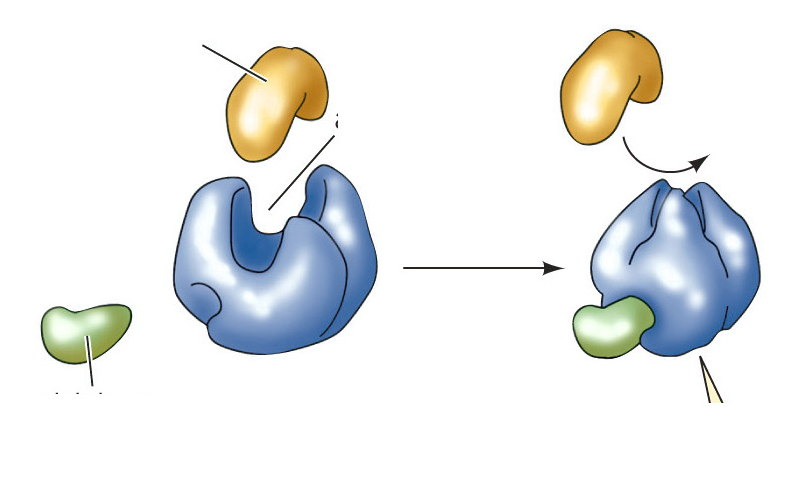
\includegraphics[width=7cm]{/share/00_SCHULE_DATA-add/bilder_saz/Purves/abbildungen/kap-06/06-18-2_v4.jpg}
		  \caption[allosteric inhibition, Purves chp 6 fig 06-18-2]{Visualisation of \textbf{allosteric} inhibition of an enzymatically catalysed reaction}
		  \label{fig:AllostericInhibition}
		%\setfloatalignment{b}
		\end{figure}

\subsubsection{Regulation of enzyme activity through competitive inhibition }
	\begin{enumerate}[resume, leftmargin=*]
\item  Unfortunately, Starr doesn't explain you the concept of ``competitive inhibition``. Study figure \ref{fig:CompetitiveInhibition} and figure out, what this process is all about:\\
	\Loesung{... has to be yet written...}{1.1 cm}
\end{enumerate}				

		\begin{figure}[htp]
		  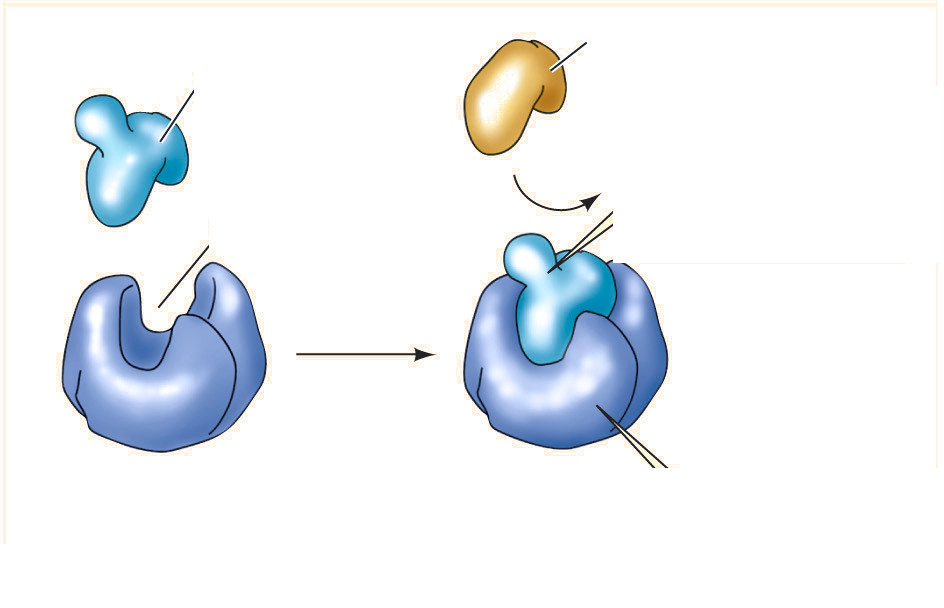
\includegraphics[width=8cm]{/share/00_SCHULE_DATA-add/bilder_saz/Purves/abbildungen/kap-06/06-18_v2.jpg}
		  \caption[allosteric inhibition, Purves chp 6 fig 06-18\_v2]{ Visualisation of \textbf{competitive} inhibition of an enzymatically catalysed reaction}
		\label{fig:CompetitiveInhibition}
		%\setfloatalignment{b}
		\end{figure}
		

		\vspace{2cm} \enlargethispage{1.8cm}
\subsubsection{Feedback inhibition}
		\begin{enumerate}[resume, leftmargin=*]
\item  Read \ding{229} Starr (9ed), chp 5.4 and then explain the concept of \emph{feedback inhibition}!\\
	\Loesung{ feedback inhibition describes how products of foregoing enzymatic reactions may alter a subsequent reaction

	\vspace{0.1cm}
	\includegraphics[width=10cm]{/share/00_SCHULE_DATA-add/Starr/Starr-9ed_res/chapter05/starr05-016.jpg}
	}{2cm}
\end{enumerate}		
\clearpage

% 			
% 	\textcolor{white}{...}
% 	\vspace{4pt}
% 	\begin{minipage}[htbp]{16cm}
% 	\centering {\includegraphics[width=16cm]{/share/SB_Unterricht/Biology/met02_enzymes/EnzymesConceptMap.png}} \captionof{figure}[Enzyme concept map (sse www-bozeman)]{General concept of processes involved in enzyme activity. See figure \ref{fig:EnzymeSubstrateCompetitor} - the top sub figure - for a general model of enzymatic cleavage!}  	\label{fig:EnzymesConceptMap}
% 	\vspace{2cm}
% 	\end{minipage}	
% 	
% 
% 		\piccaptionoutside 					
% 		%\setcapmargin*[-2cm ]{0cm }  
% 		\piccaption[Regulation of an allosteric enzyme - activation and inhibition; Schroedel SII, p.60, Fig. 1]{\label{fig:EnzymeRegulatoryCenters} Enzymes may be positively or negatively regulated - activated or inhibited.}    
% 		\parpic[l]{\includegraphics[width=12cm]{/share/SB_Unterricht/Biologie/met02_Enzyme/SchroedelSII_p60_enzym_v3.png}}
% 		\picskip{0}
% 		%\setcapmargin*[0cm ]{0cm }	
		
%   \areaset[0cm]{11.5cm}{26.5cm}  			
		
		
	\clearpage
  \areaset[0cm]{11.5cm}{26.5cm}  
% 				

	\subsubsection{Exercises and calculations}
				\begin{enumerate}[itemsep=1.5em, leftmargin=*]

\marginline{ \vspace{3cm}
		 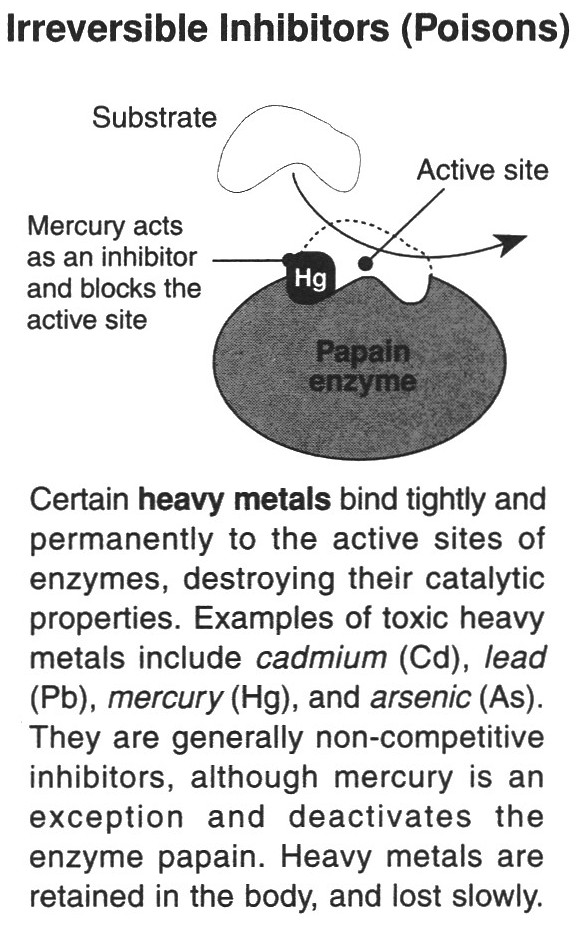
\includegraphics[width=5cm]{/share/00_SCHULE_DATA-add/Buecher_Bio/biozone/cells/BioZone_cells_p028-3_v2.jpg}}	

		 		\item  The enzyme pepsin is found in the stomach. Would it function in the small intestine as well? Formulate a reasonable hypothesis!
				\Loesung{\\ pH value in the stomach is very low, about pH 1; pH in the small intestine is neutral, or slightly acidic, about pH 7.6 } {1.2cm}

				\item A given enzyme works faster if warmed - double the speed for an increase of 10°C. Why does the same enzyme slow down, when heated 30°C above its normal range?
				\Loesung{\\ enzymes are proteins; heat destroys the 3-D structure, the quart. and tert. structures of proteins. }{2cm}
		
				\item Repeat the concepts enzymatic activity and its inhibtion: \hrefL{/share/SB_Unterricht/Biology/met02_enzymes/Enzyme_Animation.mp4}{https://www.dropbox.com/s/7pwjuofi68304a8/Enzyme_Animation.mp4?dl=0}{film link: Enzyme\_Animation.mp4}
				
				
				
				\item Explain why paints containing Cadmium or other heavy metals were expelled from sale and use! Famous painter VanGogh didn't know about these problems and developed a heavy neural illness. What do we learn from VanGoghs' fate? More on this: \href{http://en.wikipedia.org/wiki/Vincent_van_Gogh\%27s_health}{Wikipedia, VanGogh, health - see "`lead poisoning"'}
					
	\marginline{ 
		 \includegraphics[width=3.5cm]{/share/SB_Unterricht/Biologie/met02_Enzyme/SchroedelSII_p58-1_enzym_v2.png}}
% 		 \captionof{figure}[VERZEICHNIS]{LEGENDE}
% 	         \label{fig:LABEL} }
					
% 	\vspace{4pt}
% 	\begin{minipage}[htbp]{1\columnwidth}
% 	\centering {\includegraphics[width=5.5cm]{/share/00_SCHULE_DATA-add/Buecher_Bio/biozone/cells/BioZone_cells_p028-3_v1.jpg}}
% 	\vspace{2pt}
% 	\end{minipage}
				
				\item Explain the graph "`Reaktionsgeschwindigkeit"' over "`Substratkonzentration"' by help of the three small pictures in the margin (\textit{Randspalte}).
				
				
	\vspace{4pt}
	\begin{minipage}[htbp]{1\columnwidth}
	\centering {\includegraphics[width=8cm]{/share/SB_Unterricht/Biologie/met02_Enzyme/SchroedelSII_p58-2_enzym_v2.png}} \captionof{figure}[Rekationsgeschw. in Abhängigkeit der Substratkonzentration aus Schroedel SII]{The \textbf{rate of a reaction} (\textit{dt: Reaktionsgeschwindigkeit}) depends on \textbf{substrate concentration} (\textit{dt: Substratkonzentration}) }  	\label{fig:ReactionrateSubstrateConc}
	\vspace{2pt}
	\end{minipage}
				
				
	\clearpage			
			\item An enzyme shows inhibition in the presence of a specific agent. Plotting the reaction rates in response to this agent allows for the identification of the kind of inhibition - competitive or allosteric. Describe figure \ref{fig:ReversibleHemmung} in your own words.
			
		
	\vspace{4pt}
	\
	\begin{minipage}[htbp]{16cm}
	\centering {\includegraphics[width=16cm]{/share/SB_Unterricht/Biologie/met02_Enzyme/SchroedelSII_p58-3_enzym_v1.png}} \captionof{figure}[Zwei Typen reversibler Hemmung, aus SchroedelSII p58]{Reversible inhibition might be competitive (A) or non-competitive (B)}  	\label{fig:ReversibleHemmung}
	\vspace{2pt}
	\end{minipage}
				
				
	\item Please find below some more exercises on enzymatic reactions (\textit{taken from the biozone workbook}):

	\enlargethispage{2cm}
\begin{minipage}{15cm}
\begin{multicols*}{2}
		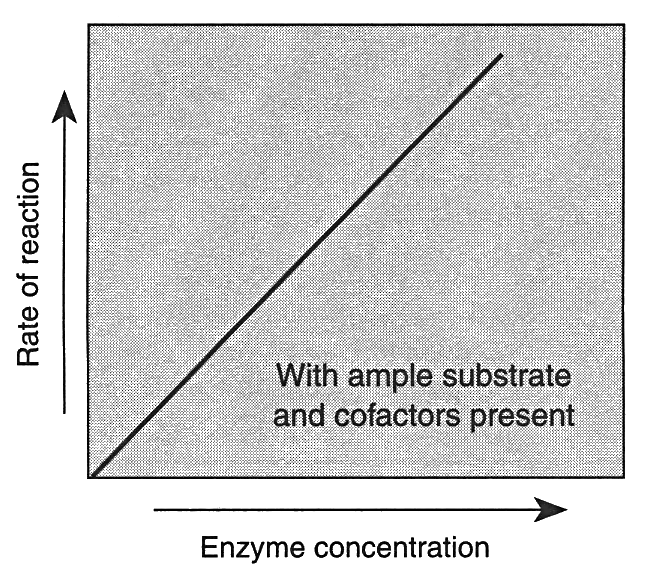
\includegraphics[width=0.8\columnwidth]{/share/00_SCHULE_DATA-add/Buecher_Bio/biozone/cells/BioZone_cells_p027_v1.png}
	\vfill\null
	\columnbreak
		 \textbf{Enzyme concentration}
	 		\begin{enumerate}[label=\textit{(\arabic*)},leftmargin=0em,series=zaehler]
		      \item Describe the change in the rate of reaction when the enzyme concentration is increased (assuming there is plenty of the substrate present):
			      \Loesung{\\linear increase of the reaction rate with concentration of the enzyme}{1.2cm}
		      \item  Suggest how a cell may vary the amount of enzyme present in a celI: 
			      \Loesung{\\ Trough the production of enzymes (proteins...) or throuhg the break down of (old) enzymes.}{1.2cm}
		      \end{enumerate}
	\end{multicols*}
\end{minipage}

\begin{minipage}{15cm}
\begin{multicols*}{2}
		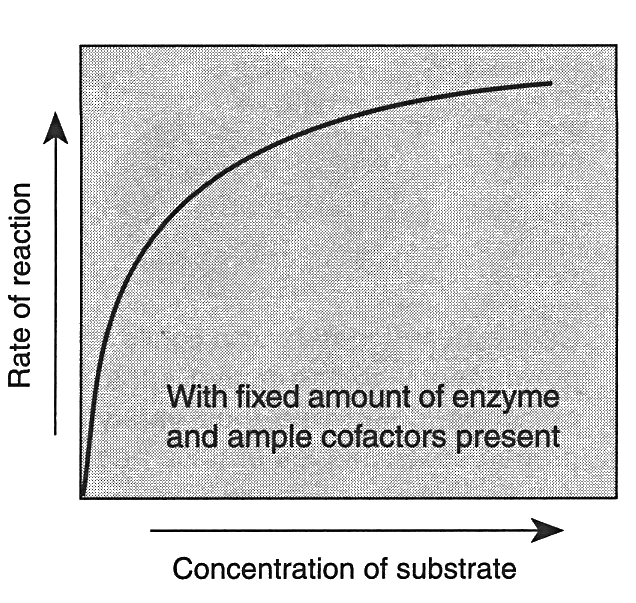
\includegraphics[width=0.8\columnwidth]{/share/00_SCHULE_DATA-add/Buecher_Bio/biozone/cells/BioZone_cells_p027_v2.png}
	\vfill\null
	\columnbreak
			 \textbf{Substrate concentration}
	 		\begin{enumerate}[label=\textit{(\arabic*)},leftmargin=0em,series=zaehler]
		      \item  Describe the change in the rate of reaction when the substrate concentration is increased (\textit{assuming a fixed amount of enzyme and enough of evtl. required cofactors}):
			      \Loesung{\\ At first a steep increase in reaction rate can be observed; followed by a slow down of the increase; finally reaching a constant reaction rate.}{1.8cm}
		      \item  Explain why the rate changes the way it does:
			      \Loesung{\\ Each conversion of a substrate requires a certain time span. As soon as every enzyme molecule is being constantly active without having to wait for a substrate molecule to arrive at the active site, the maximum rate of reaction is reached (\textit{= horizontal line}).}{1.8cm}
		      \end{enumerate}
	\end{multicols*}
\end{minipage}

\hspace{-3cm}
\begin{minipage}{15cm}
\begin{multicols*}{2}
		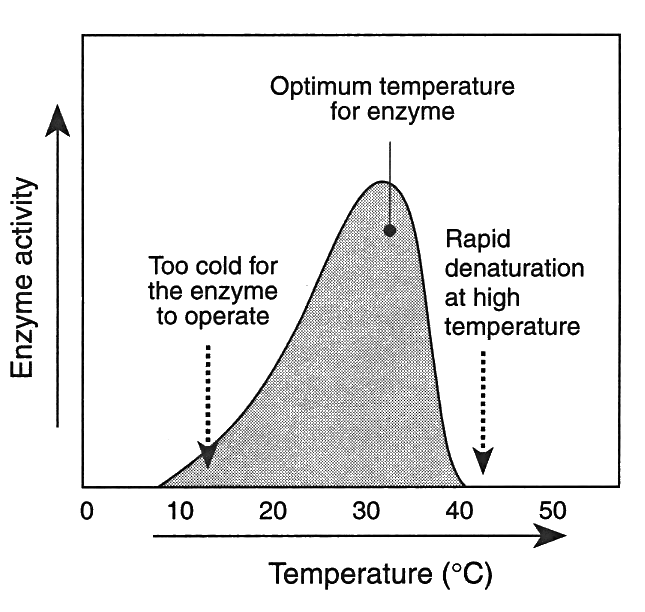
\includegraphics[width=0.8\columnwidth]{/share/00_SCHULE_DATA-add/Buecher_Bio/biozone/cells/BioZone_cells_p027_v3.png}
	\vfill\null
	\columnbreak
			 \textbf{Temperature}\\
			 Higher temperatures speed up all reactions, but few enzymes can tolerate temperatures higher than $50 - 60\,\celsius$. The rate at which enzymes are denatured (change their shape and become inactive) increases with higher temperatures.
	 		\begin{enumerate}[label=\textit{(\arabic*)},leftmargin=0em,series=zaehler]
		      \item 
		       Describe what is meant by an optimum temperature for enzyme activity:
			      \Loesung{\\ The temperature at which an enzyme performs best (to asses this, substrate- and enzyme-concentrations have to be kept constant)}{1.8cm}
		      \item  Explain why most enzymes perform poorly at low temperatures:
			      \Loesung{\\ The lower the temperature, the slower the \emph{molecular movement} ("`Brown's particle movement"') and thus the threshold of the activation energy is less likely to be reached by a particular substrate molecule.}{2.6cm}
		      \end{enumerate}
	\end{multicols*}
\end{minipage}

\vspace{1cm}
\hspace{-3cm}
\begin{minipage}{15cm}
\begin{multicols*}{2}
		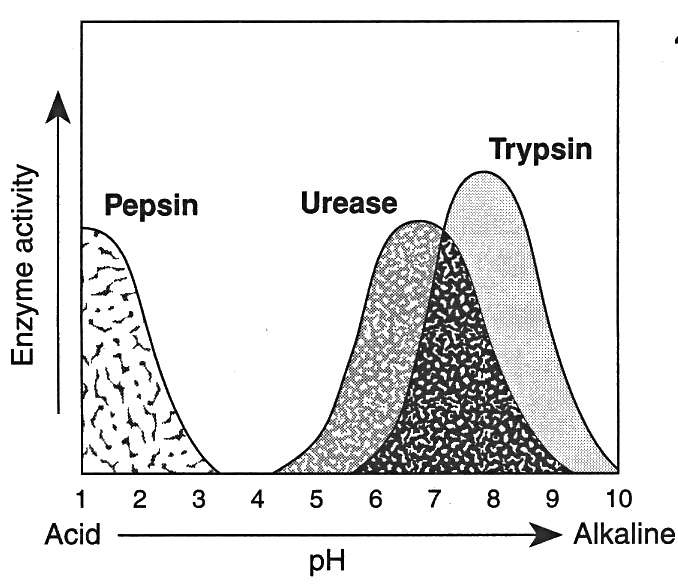
\includegraphics[width=0.8\columnwidth]{/share/00_SCHULE_DATA-add/Buecher_Bio/biozone/cells/BioZone_cells_p027_v4.png}
	\vfill\null
	\columnbreak
		 \textbf{pH (acidity / alkalinity}
		 Like all proteins, enzymes are denatured by extremes of pH (very acid or alkaline). Within these extremes, most enzymes are still influenced by pH. Each enzyme has a preferred pH range for optimum activity.
	 		\begin{enumerate}[label=\textit{(\arabic*)},leftmargin=0em,series=zaehler]
		      \item  State the optimum pH for each of the enzymes: \\
			      Pepsin: \gap{pH 1.5}; Trypsin: \gap{pH 8} Urease: \gap{pH 6.5}
		      \item Pepsin acts on proteins in the stomach. Explain how its optimum pH is suited to its working environment:
			      \Loesung{\\ The gastric fluid is highly acidic due to HCl (given off by the parietal cells). Most proteins are denatured at the very low pH in the stomach. Pepsin needs to be a very specific kind of protein in order to stay active at pH 1.5!}{1.8cm}
		      \end{enumerate}
	\end{multicols*}
\end{minipage}
				
				
								
				\end{enumerate}
	
		
% 
% \includepdf[pages=20-20,clip=true,scale=0.95, pagecommand=\pagestyle{headings}, viewport=0cm 1.1cm 20cm 24cm, addtotoc={
%      20,subsubsection,3,EnzymeReactionRate exerc.,p1}]	% last p -entry NO COMMA!
%      {/share/00_SCHULE_DATA-add/Buecher_Bio/biozone/cells/biozone_cells_008-028_ocr-2.pdf}  


%********************************************************************

\clearpage
\subsection{Lab work: Quantitative Enzyme Studies with Catalase}

\subsubsection*{Objectives}
In this exercise you will study the enzyme catalase, which accelerates the breakdown of hydrogen peroxide (a common end product of oxidative metabolism) into water and oxygen, according to the summary reaction:

\ce{2H2O2 + catalase -> 2H2O + O2 + catalase}

This catalase-mediated reaction is extremely important in the cell because it prevents the accumulation of hydrogen peroxide, a strong oxidizing agent which tends to disrupt the delicate balance of cell chemistry.

Catalase is found in animal and plant tissues, and is especially abundant in plant storage organs such as potato tubers, corms, and in the fleshy parts of fruits. You will isolate catalase from potato tubers and measure its rate of activity under different conditions. A glass, fiber filter will be immersed in the enzyme solution, then placed in the hydrogen peroxide substrate. The oxygen produced from the subsequent reaction will become trapped in the disc and will give it buoyancy. The time measured from the moment the disc touches the substrate to the time it reaches the surface of the solution is a measure of the rate of the enzyme activity.


\subsubsection*{Materials and solutions}
You'll be provided with all the lab equipment as well as 100\,\milli\litre of freshly made potato extract per group.
	\todo{some glass ware doesn't correspond with the manual given here!}

\subsubsection{Test 1: Effect of Enzyme Concentration}
Before considering the factors which affect enzyme reactions, it is important to demonstrate that the enzyme assay shows that the enzyme actually follows accepted chemical principles. One way to demonstrate this is by determining the effect of enzyme concentration on the rate of activity, while using a substrate concentration which is in excess.

Label four 50-ml beakers as follows: 100, 75, 50, and 25 units/per ml. Prepare 40 ml of enzyme for each of the concentrations:

% 	\begin{table}[!htbp]
	\begin{center}
	\setlength{\extrarowheight}{2pt}
% 	\captionof{table}[VERZEICHNIS]{TABELLENUEBERSCHRIFT}
	  \vspace{12pt}  \hspace{0cm}
	    \begin{tabularx}{10cm}[]{>\bfseries c p{1.2cm} p{1.2cm} p{1.2cm} p{1.2cm}} %
	\toprule
		 beaker & \textbf{\#E1} &  \textbf{\#E2}  & \textbf{\#E3}  &  \textbf{\#E4*}   \\\midrule
		potato extract & 10 \milli\litre  & 20  \milli\litre  & 30 \milli\litre  & >40  \milli\litre\, \tiny{(the rest})     \\
       ice water   & 30 \milli\litre & 20   \milli\litre  & 10  \milli\litre  & 0 \milli\litre     \\ \midrule
       units / \milli\litre \,\textit{\tiny{(definition)}}   & 25 &  50 & 75 & 100  \\
	\bottomrule
	\end{tabularx}%
% 	  \label{tab:TABELLENLEGENDE}%
% 	\end{table}%
	\\ \hfill *\protect{\footnotesize{save this undiluted enzyme for Tests 2 to 4}}
	\end{center}



%%% with smaller volumes:
% % Label four large test tubes (TT) as follows: 100, 75, 50, and 0 units/per ml. Prepare 10 ml of enzyme for each of the concentrations:
% %
% % % 	\begin{table}[!htbp]
% % 	 \centering
% % 	\setlength{\extrarowheight}{2pt}
% % % 	\captionof{table}[VERZEICHNIS]{TABELLENUEBERSCHRIFT}
% % 	  \vspace{12pt}  \hspace{0cm}
% % 	    \begin{tabularx}{10cm}[]{>\bfseries c p{1.2cm} p{1.2cm} p{1.2cm} p{1.2cm}} %
% % 	\toprule
% % 		 large TestTube & \textbf{\#E1} &  \textbf{\#E2}  & \textbf{\#E3}  &  \textbf{\#E4*}   \\\midrule
% % 		potato extract & 2.5 \milli\litre  & 5  \milli\litre  & 7.5 \milli\litre  & >15  \milli\litre\, \tiny{(the rest})     \\
% %        ice water   & 7.5 \milli\litre & 5   \milli\litre  & 2.5  \milli\litre  & 0 \milli\litre     \\ \midrule
% %        units / \milli\litre \,\textit{\tiny{(definition)}}   & 25 &  50 & 75 & 100  \\
% % 	\bottomrule
% % 	\end{tabularx}%
% % % 	  \label{tab:TABELLENLEGENDE}%
% % % 	\end{table}%
	% \hfill *\protect{\footnotesize{save this undiluted enzyme for Tests 2 to 4}}





Keep your catalase preparations in the ice bath. Label an identical set of beakers (\#S1 to \#S4) for the substrate. Into each of these beakers, measure out \emph{80 ml of a 1\% hydrogen peroxide} solution.

Using forceps, immerse a 4-cm (glass fiber) filter disc to one-half its diameter in the catalase solution you have prepared. Allow the disc to absorb the enzyme solution for 5 seconds, remove and drain by touching the edge to a paper towel for 10 seconds. Drop the disc into the first substrate solution. The disc will sink rapidly into the solution. The oxygen produced from the breakdown of the hydrogen peroxide by catalase becomes trapped in the fibers of the disc causing the disc to float to the surface of the solution. The time (t) in seconds, from the second the disc touches the solution to the time it again reaches the surface is determined to be the rate R of enzyme activity where R = 1/t. Repeat the procedure twice for each enzyme concentration and average the results. Record your results in the table below. Plot your results on the grid provided and label the graph.

How does enzyme activity vary with enzyme concentration?


% 		\begin{table}[!htbp]
	\begin{center}
	\setlength{\extrarowheight}{2pt}
% 	\captionof{table}[VERZEICHNIS]{TABELLENUEBERSCHRIFT}
	  \vspace{12pt}  \hspace{0cm}
	    \begin{tabularx}{10cm}[]{>\bfseries c c c c c} %
	\toprule
		  beaker & \textbf{\#S1} &  \textbf{\#S2}  & \textbf{\#S3}  &  \textbf{\#S4}   \\\midrule
		% \ce{H2O2}-solution 1\% & 80  \milli\litre  & 80 \milli\litre  & 80  \milli\litre  & 80 \milli\litre     \\
       Filter with enzyme sol.  & \#E1&  \#E2 & \#E3 &  \#E4    \\
       1. trial & \gap{95 \second}& \gap{76 \second} & \gap{57 \second} &  \gap{38 \second} \\
       2. tiral &  \gap{93 \second} & \gap{77 \second}  & \gap{59 \second} & \gap{35 \second}  \\
       3. trial &  \gap{97 \second} & \gap{74 \second}  & \gap{54 \second} & \gap{39 \second}  \\ \midrule
       average &  \gap{95 \second} & \gap{75.5 \second}  & \gap{65.5 \second} & \gap{37.5 \second}  \\
	\bottomrule
	\end{tabularx}%
	  \label{tab:TABELLENLEGENDE}%
% 	\end{table}%
	\end{center}



	\vspace{1cm}
 	\def\width{11}
	\def\hauteur{8}
	
\begin{tikzpicture}[x=1cm, y=1cm, semitransparent]
	\draw[step=1mm, line width=0.1mm, black!30!white] (0,0) grid (\width,\hauteur);
	\draw[step=5mm, line width=0.2mm, black!40!white] (0,0) grid (\width,\hauteur);
	\draw[step=5cm, line width=0.5mm, black!50!white] (0,0) grid (\width,\hauteur);
	\draw[step=1cm, line width=0.3mm, black!90!white] (0,0) grid (\width,\hauteur);
	\end{tikzpicture}

\clearpage
\subsubsection{Test 2: Effect of Substrate Concentration}
To determine the effect of substrate concentration on enzyme activity obtain eight 50-ml
beakers and label them as follows: 0\%, 0.1\%, 0.2\%, 0.5\%, 0.8\%, 1\%, 5\%, and 10\% \ce{H2O2}.
Add 40 ml of the proper (as outlined above) \ce{H2O2} solution to each beaker. Make sure that the
substrate solutions reach room temperature before beginning your assay. Using the filter disc
procedure described above, and the undiluted enzyme from Test 1, determine the rate of the reaction
at the various substrate concentrations. Record your results in the next table. Repeat the procedure
twice for each substrate concentration and average the results. Plot your results in mm-grid and
label the graph.
How is the rate of enzyme activity affected by increasing the concentration of the substrate?
What do you think would happen if you increased the substrate concentration to 20\%  \ce{H2O2}? Does
changing the substrate concentration exhibit the same effect as changing the enzyme concentration?

		\begin{table}[!htbp] \centering
	\setlength{\extrarowheight}{6pt}
% 	\captionof{table}[VERZEICHNIS]{TABELLENUEBERSCHRIFT}
	  \vspace{12pt}  \hspace{0cm}
	    \begin{tabularx}{15cm}[]{>\bfseries c  p{1.4cm} p{1.4cm} p{1.4cm} p{1.4cm} p{1.4cm} p{1.4cm}} %
	\toprule
		 beaker & \textbf{\#S11} &  \textbf{\#S12}  & \textbf{\#S13}  &  \textbf{\#S14} &  \textbf{\#S15} &  \textbf{\#S16}   \\\midrule
		  %\ce{H2O}  &78.4 \milli\litre  & 76 \milli\litre  & 73.6 \milli\litre & 72 \milli\litre & 66.7 \milli\litre& 53.4 \milli\litre   \\
		% \ce{H2O2}-Lösung 30\% & 1.6 \milli\litre   & 4 \milli\litre&6.4 \milli\litre& 8 \milli\litre  & 13.3 \milli\litre  &26.6 \milli\litre \\
		 Concentration of  \ce{H2O2} & 0.2\%   & 0.5\% &  0.8\%&1\%  & 5\%  & 10\%\\
		 1. trial & \gap{ \second} & \gap{ \second} & \gap{ \second} & \gap{ \second} & \gap{ \second} & \gap{ \second} \\
		 2. trial & \gap{ \second} & \gap{ \second} & \gap{ \second} & \gap{ \second} & \gap{ \second} & \gap{ \second} \\
		 3. trial & \gap{ \second} & \gap{ \second} & \gap{ \second} & \gap{ \second} & \gap{ \second} & \gap{ \second} \\ \midrule
		 average  &  \gap{ \second} & \gap{ \second} & \gap{ \second} & \gap{ \second} & \gap{ \second} & \gap{ \second} \\
	\bottomrule
	\end{tabularx}%
	  \label{tab:TABELLENLEGENDE}%
	\end{table}%

	\vspace{1cm}
 	\def\width{11}
	\def\hauteur{8}
	
\begin{tikzpicture}[x=1cm, y=1cm, semitransparent]
	\draw[step=1mm, line width=0.1mm, black!30!white] (0,0) grid (\width,\hauteur);
	\draw[step=5mm, line width=0.2mm, black!40!white] (0,0) grid (\width,\hauteur);
	\draw[step=5cm, line width=0.5mm, black!50!white] (0,0) grid (\width,\hauteur);
	\draw[step=1cm, line width=0.3mm, black!90!white] (0,0) grid (\width,\hauteur);
	\end{tikzpicture}

 \areaset[0cm]{18cm}{28cm}
\begin{multicols}{2}[
\subsubsection{Test 3: Effect of Enzyme Inhibitor}]
Hydroxylamine attaches to the iron atom (a part of the catalase molecule) and thereby interferes with the formation of enzyme-substrate complex. Add 5 drops of 10\% hydroxylamine to 1 ml of enzyme extract (\textit{enzyme + hydroxylamine}) and let it stand for 1 minute. Prepare a control solution (\textit{without hydroxylamine}) to test. Then measure the activity of each solution. Use two beakers (\# X1 and \# X2)  filled with 80 ml of 1\% H2O2 for the substrate each. Record data in next table Explain your results.
\end{multicols}
% 		\begin{table}[!htbp]
% 	\begin{center}
	\setlength{\extrarowheight}{2pt}
% 	\captionof{table}[VERZEICHNIS]{TABELLENUEBERSCHRIFT}
	  \vspace{12pt}  \hspace{0cm}
	    \begin{tabularx}{10cm}[]{>\bfseries c c c c c} %
	\toprule
		  beaker & \textbf{\#X1} &  \textbf{\#X2}     \\\midrule
		% \ce{H2O2}-solution 1\% & 80  \milli\litre  & 80 \milli\litre  & 80  \milli\litre  & 80 \milli\litre     \\
	       Filter with  & enzyme & enzyme + hydroxylamine   \\
       1. trial & \gap{95 \second}& \gap{76 \second}  \\
       2. tiral &  \gap{93 \second} & \gap{77 \second}   \\
       3. trial &  \gap{97 \second} & \gap{74 \second}   \\ \midrule
       average &  \gap{95 \second} & \gap{75.5 \second}   \\
	\bottomrule
	\end{tabularx}%
	  \label{tab:TABELLENLEGENDE}%
% 	\end{table}%
% 	\end{center}


\vspace{1cm}
\begin{multicols}{2}[\subsubsection{Test 4: Effect of Temperature on catalase activity}]
Using 80 ml of a 1\% hydrogen peroxide solution as the substrate, and 5-ml aliquots of the 100 units/ml enzyme solution, measure the enzyme activity in the usual manner. Therefore prepare 4 beakers (T\#1 to T\#4) Run the reactions in the water baths at different temperatures, such as 4\degreecelsius, 15\degreecelsius,  22\degreecelsius (room temperature ), 30\degreecelsius, and 37\degreecelsius. \texttt{The catalase and substrate should be brought to the testing temperature before they are used}. Record the exact temperature and your data following table and plot the results on the grid. Also test the activity of enzyme that has been boiled. (Do not boil the \ce{H2O2}!!) From these data, what can you conclude about how temperature affects enzyme activity? How would you explain the results?
\end{multicols}


% 		\begin{table}[!htbp]
	\begin{center}
	\setlength{\extrarowheight}{2pt}
% 	\captionof{table}[VERZEICHNIS]{TABELLENUEBERSCHRIFT}
	  \vspace{12pt}  \hspace{0cm}
	    \begin{tabularx}{10cm}[]{>\bfseries c c c c c} %
	\toprule
		  beaker & \textbf{\#T1} &  \textbf{\#T2}  & \textbf{\#T3}  &  \textbf{\#T4}   \\\midrule
		% \ce{H2O2}-solution 1\% & 80  \milli\litre  & 80 \milli\litre  & 80  \milli\litre  & 80 \milli\litre     \\
      run at   & 4\degreecelsius &  15\degreecelsius, & 22\degreecelsius &  30\degreecelsius    \\
       1. trial & \gap{95 \second}& \gap{76 \second} & \gap{57 \second} &  \gap{38 \second} \\
       2. tiral &  \gap{93 \second} & \gap{77 \second}  & \gap{59 \second} & \gap{35 \second}  \\
       3. trial &  \gap{97 \second} & \gap{74 \second}  & \gap{54 \second} & \gap{39 \second}  \\ \midrule
       average &  \gap{95 \second} & \gap{75.5 \second}  & \gap{65.5 \second} & \gap{37.5 \second}  \\
	\bottomrule
	\end{tabularx}%
	  \label{tab:TABELLENLEGENDE}%
% 	\end{table}%


	\vspace{1cm}
 	\def\width{9}
	\def\hauteur{6}
	
\begin{tikzpicture}[x=1cm, y=1cm, semitransparent]
	\draw[step=1mm, line width=0.1mm, black!30!white] (0,0) grid (\width,\hauteur);
	\draw[step=5mm, line width=0.2mm, black!40!white] (0,0) grid (\width,\hauteur);
	\draw[step=5cm, line width=0.5mm, black!50!white] (0,0) grid (\width,\hauteur);
	\draw[step=1cm, line width=0.3mm, black!90!white] (0,0) grid (\width,\hauteur);
	\end{tikzpicture}
\end{center}

% %*******************************************
% \subsection{Lab work: Synthesis of starch}\label{ssc:LabworkStarchSynthesis}
%
% 	\vspace{4pt}
% 	\begin{minipage}[htbp]{12cm}
% 	\centering {\includegraphics[width=0.8\linewidth]{/share/SB_Unterricht/Biology/lab01_glassware/Glassware-set01.png}} \captionof{figure}[Lab glassware from the web]{Lab glassware}  	\label{fig:glassware01}
% 	\vspace{8pt}
% 	\end{minipage}
%
%
% \enlargethispage{1.2cm}
% 	\subsubsection*{A simple test procedure to identify starch}
% 	 \todol{safe time - demonstrate this!}
% 			\begin{enumerate}[label=\textit{(\arabic*)},leftmargin=0em,series=zaehler]
% 		      \item Cut a slice of a potato. Give 2 drops of Lugol solution onto the potato slice using a medicine dropper. Describe your observations:
%
% 		      \Loesung{the potato turns black-purple \hfill \fillwithdottedlines{1cm}}{2cm}
%
% 		      \item Place 1 medicine dropper full of glucose solution in a test tube and add 2 drops of Lugol solution.  Describe your observations:
%
% 		      \Loesung{the glucose solution does not change its colour \hfill \fillwithdottedlines{1cm}}{2cm}
%
% 		      \item Summarize the characteristics of the Lugol solution:
% 		       Describe your observations:
%
% 		      \Loesung{Lugol solution is a \emph{test reagens} for starch \hfill \fillwithdottedlines{1cm}}{2cm}
% 		\end{enumerate}
%
% % \end{minipage}
% 		\clearpage
%
% \subsubsection*{Potatoes are able to synthesize starch}
% 				\setcapmargin*[0cm ]{0cm }
% 						\marginline{ %
% 			 \includegraphics[width=5.2cm]{/share/SB_Unterricht/Biology/lab01_glassware/single-items/FunnelBuechner.png}
% 			 \captionof{figure}[Buechner funnel from Wikipedia]{Conept of a Buechner funnel and Buechner flask for vacuum filtration}
% 		         \label{fig:BuechnerFunnel}
% 		         }%
%
%
%
% 			\begin{enumerate}[label=\textit{(\arabic*)},leftmargin=0em,series=zaehler]
% 		      \item \emph{Prearrangements:} Put the Buechner flask into a sink. Mount the Buechner funnel onto it - don't forget the rubber bung (\textit{ring})! Add a piece of filter paper into the funnel, moisten the filter paper and start the aspirator (\textit{dt: Wasserstrahlpumpe}).
%
% 		      \item Wash a potato and and grind half of it on a "'Glass-raffel"` until you have finely "'mashed"` potatoes.
% 				\marginline{
% 			 \includegraphics[width=5cm]{/share/SB_Unterricht/Biology/lab01_glassware/single-items/glas-raffel_v1.jpg}
% 			 \captionof{figure}[Glasraffel vom www]{Glass-raffel}
% 		         \label{fig:GlasRaffel} }
% 		      		\setcapmargin*[0cm ]{0cm }
%
% 		      \item Use  a spatula to scoop the squish (\textit{Mus}) into the Buechner funnel onto the filter paper. Rinse the "'Glass-raffel"` with a few $\milli\liter\,$ of water from the wash bottle.
%
% 		     \item Suck the liquid part of the potato squish, the \emph{filtrate}  into the Buechner flask. The dry part of the potato squish remains on top of the filter paper and is called \emph{filter cake}. \\
% 			  \Lightning	~  \hspace{1.2cm} \fbox{ \parbox{8cm}{ Work in the sink; to stop aspiration remove the sucking tube first before closing the water supply! }}\\
% 			Stopp sucking when no water trickles anymore into the Buechner flask.
%
% 			\item  Number three test tubes consecutively, from 1 to 3. Fill each with two medicine droppers full of the filtrate - make sure the volumes are equal.
%
% 			\item Use Lugol solution to test the remaining \emph{filtrate} for starch: \gap{... there is no starch to be found \hfill}
%
% 			\item Use Lugol solution to test the remaining \emph{filter cake} for starch: \gap{... there is plenty of starch to be found \hfill}
%
% 			\item Explain the findings of the Lugol tests on the filtrate and the filter cake: \gap{... starch molecules are huge polymers and thus can't pass the paper filter; therefore they remain on the filter \hfill}
%
% 			\item \emph{Test tube 1:} add 5 \milli\liter of water from the wash bottle.
%
% 			\item \emph{Test tube 2:} add  5 \milli\liter of glucose solution
% 			 \\
% 			  \Lightning	~  \hspace{1.2cm} \fbox{ \parbox{8cm}{ Please rinse the pipette with water from the bottle after use!}}
%
% 			  \item \emph{Test tube 3:} add  5 \milli\liter of glucose-1-phosphate solution (\textit{Glucose-1-Phosphatlösung}) solution
%
% 			  \item Use a vortex to mix the contents of the three test tubes (hold the glasses at the center for best results) and place all three tubes in the water bath (\textbf{40° C}).
%
% 			  \item Mix the contents of the test tubes occasionally.
% 		\end{enumerate}
%
% % 		\bgroup
% % 		\centering \fbox{ \textbf{--start with the second experiment now!--}}
% % 		\egroup
%
%
% 		\clearpage
% 		\begin{enumerate}[label=\textit{(\arabic*)},leftmargin=0em,series=zaehler,resume]
% 		 \item After 15 minutes (or later) ad two drops of Lugol solution to each of the three test tubes \fbox{observe immediately!} and gently agitate the test tubes.
%
% 		 \item Describe your observations:
% 			 \begin{itemize}
% 			  \item \emph{Test tube 1:} \gap{... no changeof the Lugol colour: Lugol test negative   $\rightarrow$\textbf{ no} starch present  \hfill}
% 			  \item \emph{Test tube 2:}\gap{... no change of the Lugol colour: Lugol test negative  $\rightarrow$ \textbf{no} starch present \hfill}
% 			  \item \emph{Test tube 3:} \gap{... Lugol turns black: Lugol test positive $\rightarrow$ \textbf{some} starch present \hfill}
% 			 \end{itemize}
%
% 		\item You could observe a difference in test tube 2 and 3. Refer in your argumentation to the theory about enzymes:
% 			\Loesung{\\ substrate specificity }{3.2cm}
%
% 		\item What is the role of the phosphate present in \emph{glucose-1-phophate}? Refer in your argumentation to the theory about cell respiration:
% 			\Loesung{\\ activation of the glucose using phophate - alike the ADP plus P to ATP story }{3.2cm}
%
% 		\item Summarize the findings of the experiment done:
% 				\Loesung{\\ substrate specificity of enzymes \\
% 				 and need of activation of building blocks to make a polymer }{3.2cm}
% 		\end{enumerate}
%
%
%
%
%
%     \clearpage
% \subsection{Lab Work: Investigate the activity of Urease }
% \subsubsection*{Methyl-Red is a pH indicator}
% 	pH-indicators are substances that can quickly tell us the pH of a liquid
%
%
% 	pH 7 is \emph{neutral}, pH < 7 is \emph{acidic},  pH > 7 is \emph{alkaline}\\
% 	e.g. lemon juice shows pH 2-3, CocaCola shows pH 2, vinegar reaches to pH 4-5, skin pH is around 5-6, pH of clean water is around pH 7 to pH 8, classical soap is alkaline with pH 9, hydrogen oxid  \ce{OH-} reaches up to pH 14 which is the upper end of the pH scale
%
% 	Give two fingers high of water (2 ml ) into a test tube  and add a drop of \textbf{methyl red}. \\
% 		Note the color \gap{yellow (evtl. orange)}; thus pH is \gap{> 6.2 }.
%
% 		\marginnote{\textbf{\faEyedropper ~Methyl Red indicates:}
% 	\begin{itemize}
% 		\item pH < 4.4 = red
% 		\item pH 4.4 - pH 6.2 = orange
% 		\item pH > 6.2 = yellow
% 	\end{itemize}
% 	\href{/share/SB_Unterricht/Biologie/met02_Enzyme/Methylrot-Wikipedia_Farbe.jpg}{link to color-pict}
% 	}
%
% 	Now add a drop of acetic acid to your test tube with the indicator and look what happens:\\
% 		Note the color \gap{red (evtl. orange)}; thus pH is \gap{< 4.4 }.
%
% 	Finally you add a drop of odium hydroxide solution to your test tube and look what happens:\\
% 		Note the color \gap{yellow (no orange at all!)}; thus pH is \gap{>> 6.2 }.
%
% 		 \fbox{\parbox[c][1cm][c]{12cm}
% 	{\centering
% 	The \textbf{pH-value} depends on the number of \textbf{  \ce{H+} ions}.
%
% 	The higher the number of   \ce{H+}, the lower the pH-value: pH indicates the \textsc{negative logarithme} of the number of  \ce{H+} ions.
% 	}}%
%
%
% \vfill
% \subsubsection*{Urease is an urea splitting enzyme}
%
% An enzyme's name usually refers to its substrate and the kind of reaction the enzyme catalyses. In the case of \textbf{urease}, the substrate is \textsc{urea} (Dt \textit{Harnstoff}) and the reaction is a \textsc{splitting} reaction, hence the suffix \textbf{-ase} (\textit{however, -ase is just the most general term to indicate a molecule to be an enzyme}). See the box below for the chemical reaction urea undergoes with urease.
%
% Structurally highly likely is \textbf{thiourea}. The prefix \textsc{thio} stands for sulfur and thus the molecule would be more easily recognisable as \textit{thio-urea}. See the box below for similarities and differences of the two molecules. Now you are going run an experiment to explore the reactivity of thiourea as a substrate with the urease enzyme!
%
%   \vfill
%       \enlargethispage{0.4cm}
% %        \begin{addmargin*}[0cm]{-4.4 cm}
% 	\hspace{-3cm}
%        \fbox{\parbox[c][5cm][c]{15cm}
% 	{\centering
% 	\chemfig{	O=C([::60]-NH2)([::300]-NH2)} \quad urea \hspace{2cm} \chemfig{ S=C([::60]-NH2)([::300]-NH2)} \quad thiourea
%
% 	\vspace{1cm} \flushleft \quad
% 	\ce{CO(NH2)2 + H2O ->[Urease] CO2 + 2 NH3} %\flushright
%
% % 	\vspace{0.4cm}
% 	\hspace{6cm}
% 						\ce{NH3 + H2O ->[spontaneous] NH4+ + OH-}
%
% 	}}%
% %       \end{addmargin*}
%
%
%
% \clearpage
% \subsubsection*{Urease in reaction with urea (\textit{Harnstoff}) or thiourea (\textit{Thio-Harnstoff})}
%
% 			\begin{enumerate}[label=\textit{(\arabic*)},leftmargin=0em,series=zaehler]
% 		      \item Label 6 test tubes from 1 to 6; put the tubes into the rack
%
% 		      \item Put 3 boiling stones (\textit{Siedesteinchen}) into a test tube "'DURAN"` (written on the glass) an add 2 medicine droppers (\faEyedropper) full of urease (enzyme) suspension.
%
%  \marginline{~~\includegraphics[width=2cm]{/share/SB_Unterricht/Biologie/lab01_LaborAllgmein/safetyglass.png}	}
%
% 		      \item Gently heat your urease mixture to a boil - work carefully, directing the opening of your tube towards an empty space!
%
% 		      \item Prepare all the other tubes according to the \emph{instructions} given in table \ref{tab:UreaseExperimentalSetup}.
%
% 		      \item After ten minutes reaction time note the colour of your reaction and estimate the pH according to the indicator's colour!
%
% 		      \item Draw your conclusions!
%
% 		      \end{enumerate}
%
%       \hspace{-2cm}
% %        \begin{addmargin*}[0cm]{-4 cm}
% 	\begin{minipage}{16cm}
% 	\setlength{\extrarowheight}{6pt}
% 	\captionof{table}[Table of the urease experimental setup]{Your experimental setup - work from top to bottom through this table.}
% 	  \vspace{12pt}  \hspace{0cm}
% 	    \begin{tabularx}{16cm}[]{p{5cm} c c c c c c } %
% 	    % X p{1.5cm}p{1.2cm}p{1.2cm}p{1.2cm}p{1.2cm}p{1.2cm}
% 	\toprule
% 	\textbf{Instruction}  & ~\textbf{TT-1}~  &~  \textbf{TT-2} ~ & ~ \textbf{TT-3} ~ & ~ \textbf{TT-4} ~ & ~ \textbf{TT-5} ~ & ~ \textbf{TT-6}~ \\\midrule
% 	volume of thiourea &  $5\,\milli\litre$ &  $5\,\milli\litre$ &   &   &     \\
% 	volume of urea  &   &   &  $5\,\milli\litre$ & $5\,\milli\litre$  &  $5\,\milli\litre$  &  $5\,\milli\litre$  \\
% 	volume of methyl red  & $3 \,$\begin{tikzpicture}
% % \foreach \i in {1,...,10}
%   \path  pic {raindrop};
% \end{tikzpicture}   & $3 \,$\begin{tikzpicture}
% % \foreach \i in {1,...,10}
%   \path  pic {raindrop};
% \end{tikzpicture}  & $3 \,$\begin{tikzpicture}
% % \foreach \i in {1,...,10}
%   \path  pic {raindrop};
% \end{tikzpicture}  & $3 \,$\begin{tikzpicture}
% % \foreach \i in {1,...,10}
%   \path  pic {raindrop};
% \end{tikzpicture}  & $3 \,$\begin{tikzpicture}
% % \foreach \i in {1,...,10}
%   \path  pic {raindrop};
% \end{tikzpicture} &  $3 \,$\begin{tikzpicture}
% % \foreach \i in {1,...,10}
%   \path  pic {raindrop};
% \end{tikzpicture} \\
% 	initial colour: & \ldots & \ldots &\ldots & \ldots&\ldots & \ldots \\
% % 	pH-Wert auf leicht sauer (pink)  & \textquestiondown\,  \faEyedropper \, ? &  \textquestiondown\,  \faEyedropper \, ?   &   \textquestiondown\,  \faEyedropper \, ?  &  \textquestiondown\,  \faEyedropper \, ?   &  \textquestiondown\,  \faEyedropper \, ?  &   \textquestiondown\,  \faEyedropper \, ?  \\
% 	place on ice   &   &   &   &   & X  &   \\
% 	volume of \textsc{boiled} urease   &   &   &   & $1\,\milli\litre$  &  &   \\
% 	volume of urease   & $1\,\milli\litre$  &   &  $1\,\milli\litre$ &   & $1\,\milli\litre$  &  \\
% 	water bath $40 \degree\, C$ for $5\, \minute $  &  X & X  & X  &  X &   & X \\ \midrule
% 	\textbf{results}  & & & & &  & \\
% 	end colour after (10 \minute) & \ldots & \ldots &\ldots & \ldots&\ldots & \ldots \\
% 	end pH (approximative)) & \ldots & \ldots &\ldots & \ldots&\ldots & \ldots \\
% 	\bottomrule
% 	\end{tabularx}%
% 	  \label{tab:UreaseExperimentalSetup}%
% 	      \end{minipage}
% % 	  \end{addmargin*}
%
% %       \randnotiz{Text im Rand, der auch umgebrochen wird und in einer umrandeten Box steht}
%
%
% %      \vspace{2cm}
% %       \bgroup \huge       \Pointinghand    \egroup   \textit{this experiment is under construction - you shall receive additional instructions for this lab session}
% %
% \vspace{0.4cm}
%     \bgroup \large       \Writinghand   \egroup \bgroup \Large \quad Discussion of your urease experiment \egroup % \paragraph{}
%
%     \enlargethispage{2cm}
%     \Loesung{ The expected results:
%     \begin{itemize}
%     	\item TT1: NO effect - thiourea is structural analog of urea but doesn't match the enzyme's active site.
%     	\item TT2: NO effect - no urease = no reaction possible.
%     	\item TT3: YES colour changed from red to yellow - reaction took place.
%     	\item TT4: NO effect - boiling has denatured the urease (a protein!)
%     	\item TT5: NO / weak effect - cooling slowed down the urease' activity!
%     	\item TT6 NO effect - no urease = no reaction possible.
%     \end{itemize}
% 	> This experiment demonstrates both \textbf{substrate specificity} and \textbf{temperature dependency} of an enzyme <
%     }{5cm}
%
%
%
% % 	 \areaset[2cm]{15cm}{27cm}
% % 	 \setlength{\marginparwidth}{0.9\marginparwidth}
